\chapter{Ergebnisse} \label{ergebnisse}
In dieser Arbeit wurde versucht, die hauptsächlich in der 3D-Animation verwendete Technik der skelettbasierten Animation auf 2D-Charaktere zu übertragen, um dynamisch Laufbewegungen zu erzeugen. Allgemein kann festgestellt werden, dass dieser Versuch erfolgreich war. Das entwickelte System verwendet ein Skelett und erstellt anhand einiger zuvor festgelegter Splines für jeden Schritt eine neue Bewegungsabfolge. Wird ein Mesh erstellt und seinen einzelnen Vertices Knochen zugeteilt, werden die Vertices und die darauf gezeichnete Textur anhand des Skeletts verformt.

Der Charakter verfügt dabei über die Möglichkeit, anhand der Auslenkung des Control-Sicks präzise seine Schrittweite und Bewegungsgeschwindigkeit anzupassen. Beispiele für eine langsame und eine schnelle Bewegungsanimation sind in Abb. \ref{even_slow} bzw. Abb. \ref{even_fast} zu sehen. Die Interpolation zwischen zwei verschiedenen Splines -- einem für das langsame Gehen, einem für das Rennen -- sorgt dabei dafür, dass nicht nur die Länge des Schritts wächst, sondern auch die Form der Bewegung sich verändert.

Des Weiteren wurde das Ziel erreicht, Bewegungen über Flächen verschiedener Höhen möglich zu machen. Der Charakter sucht sich dabei an der gewünschten nächsten Fußposition den passenden Boden und berechnet einen Spline mit dem entsprechenden Punkt als Ziel. Eine Animation für das Hinaufsteigen einer Stufe wird in Abb. \ref{uphill} gezeigt, das Gegenstück für das Hinabsteigen einer solchen ist in Abb. \ref{downhill} zu sehen. Eine entscheidende Limitierung ist dabei jedoch, dass gerade bei kleinen Schritten mangels Collision Detection für die Splines nicht sichergestellt werden kann, dass die dynamisch erstellten Bewegungen nicht mit dem Level kollidieren, wie in Abb. \ref{clip_through_ground} gezeigt.

Um dem Ziel der Responsivität gerecht zu werden, ist es dem Charakter möglich, auch mitten in einem Schritt abrupt stehen zu bleiben. Da ein solches plötzliches Stoppen in der Realität jedoch nicht ohne Weiteres möglich ist, könnte dies zu einer unglaubwürdigen Animation führen. Um mit diesem Problem umzugehen, wird die Bewegung des Charakters zwar sofort gestoppt, es wird aber eine Übergangsanimation eingefügt, um die Abruptheit etwas zu verschleiern. Zum stehen kommen kann der Charakter dabei auch auf unebenem Untergrund und wählt seine Pose dabei stets so, dass seine Beine sauber auf dem Boden stehen (siehe Abb. \ref{standing_uneven}).\footnote{Ein angemessenes Level wird dabei vorausgesetzt. Sind die Unterschiede zwischen benachbarten Untergründen zu groß, um realistisch auf ihnen stehen zu können, entstehen fehlerhafte Animationen.}

Außerdem werden diverse Möglichkeiten geboten, die Generierung der Animationen anzupassen. Durch die Veränderung von Schrittweite, dem Grad des Einlehnens in die Bewegungsrichtung und der Geschwindigkeit der Interpolation auf den errechneten Splines sind bereits einige Stellschrauben gegeben. Weiterhin wird aber auch noch der Spline-Editor angeboten, der die präzise Anpassung der einzelnen Splines ermöglicht, die wiederum die Grundlage der dynamisch gebildeten Animationen darstellen. Die Kombination dieser Anpassungsmöglichkeiten erlaubt dem Nutzer, eine Vielzahl von verschiedenen Bewegungsmustern für die zu animierenden Charaktere zu erstellen.

\begin{figure}
    \centering
    \begin{subfigure}[t]{.4\linewidth}
        \centering
        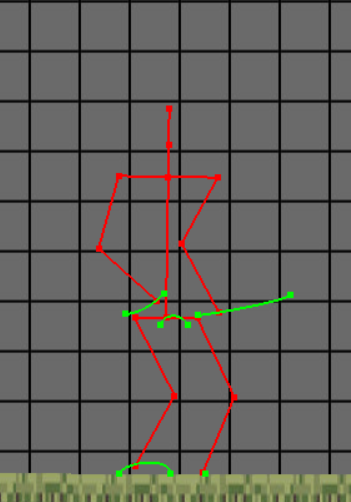
\includegraphics[width=0.75\linewidth]{images/even_ground_slow.png}
        \caption{Gehen auf ebenem Untergrund.}
        \label{even_slow}
    \end{subfigure}
    \begin{subfigure}[t]{.4\linewidth}
        \centering
        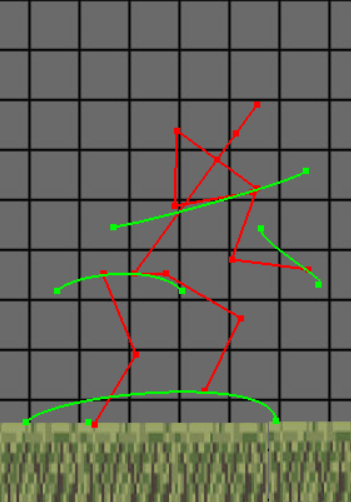
\includegraphics[width=0.75\linewidth]{images/even_ground_fast2.png}
        \caption{Rennen auf ebenem Untergrund.}
        \label{even_fast}
    \end{subfigure}
    \begin{subfigure}[t]{.4\linewidth}
        \centering
        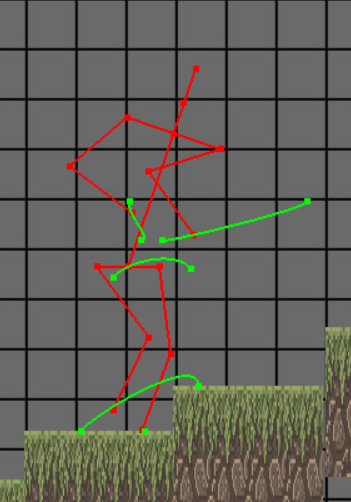
\includegraphics[width=0.75\linewidth]{images/going_up3.png}
        \caption{Bewegung bergauf.}
        \label{uphill}
    \end{subfigure}
    \begin{subfigure}[t]{.4\linewidth}
        \centering
        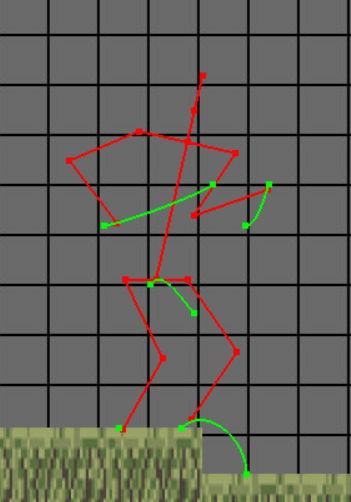
\includegraphics[width=0.75\linewidth]{images/going_down1.png}
        \caption{Bewegung bergab.}
        \label{downhill}
    \end{subfigure}
    \begin{subfigure}[t]{.4\linewidth}
        \centering
        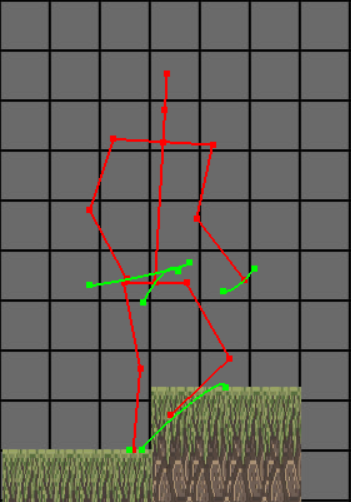
\includegraphics[width=0.75\linewidth]{images/clip_through_gorund.png}
        \caption{Ein Bein bewegt sich beim aufwärts gehen durch den Boden.}
        \label{clip_through_ground}
    \end{subfigure}
    \begin{subfigure}[t]{.4\linewidth}
        \centering
        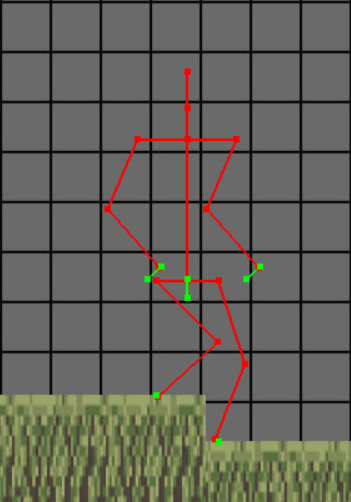
\includegraphics[width=0.75\linewidth]{images/standing_uneven.png}
        \caption{Stehen auf unebenem Untergrund.}
        \label{standing_uneven}
    \end{subfigure}
    \caption{Beispiele generierter Animationen. Das Skelett ist in rot dargestellt. Die grünen Linien stellen die Splines dar, an denen sich die entsprechenden Knochen entlang bewegen.}
\end{figure}
